% Prologue
\part*{Le Début de la Quête}
\addcontentsline{toc}{part}{Le Début de la Quête}
\markboth{Le Début de la Quête}{Le Début de la Quête}

\begin{figure}[H]
    \center
    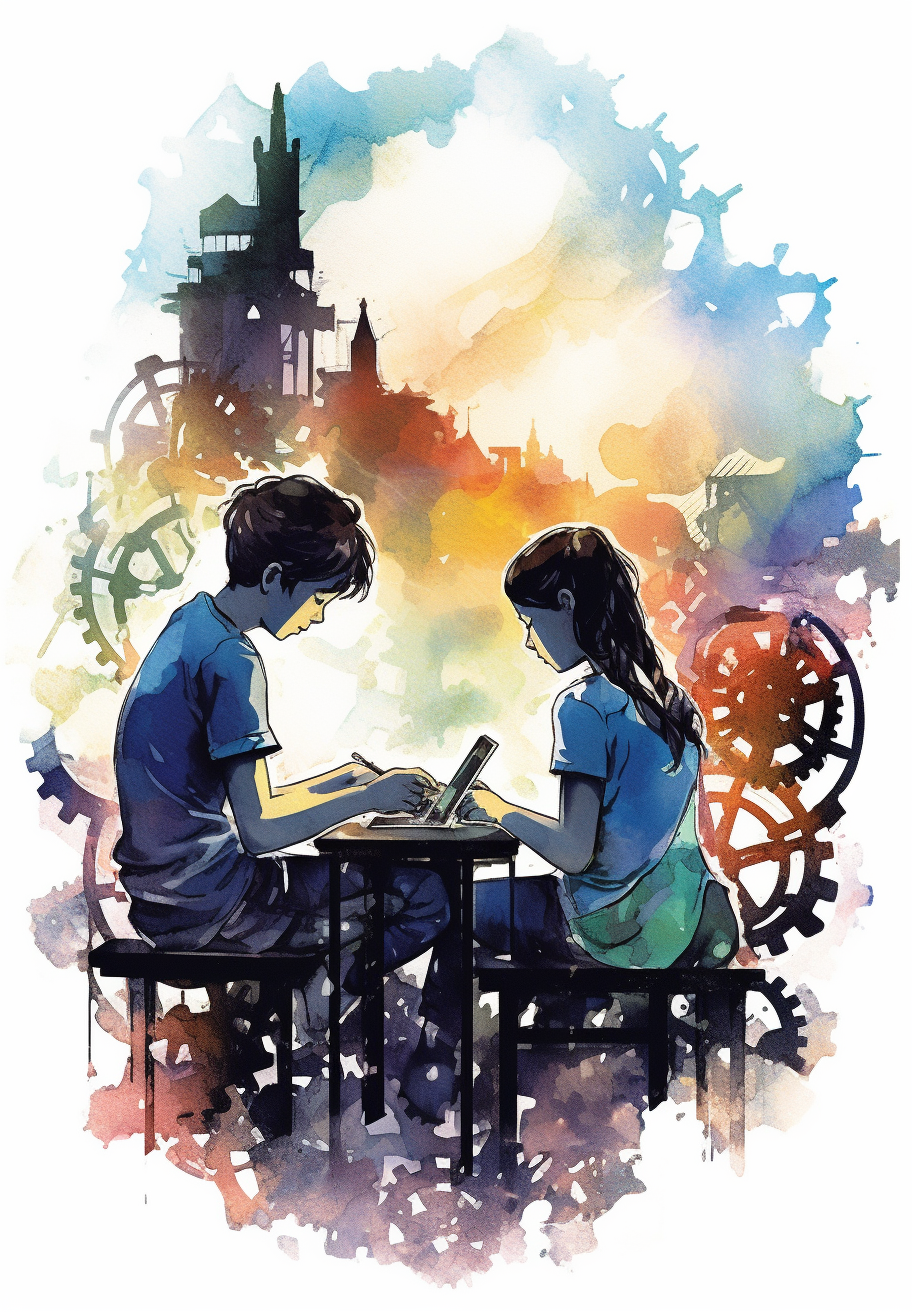
\includegraphics[keepaspectratio, width=\textwidth, height=\textheight]{images/ba90af04-6a67-48cf-bba7-51b2a346c7a6.png}
\end{figure}

Jeune développeur·euse, vous vous tenez sur le seuil d'un monde nouveau, vibrant d'opportunités et bourdonnant de potentiel. Les couloirs éthérés de l'Internet retentissent de l'écho de milliers de développeur·euse·s, écrivant et partageant du code, construisant des mondes virtuels, repoussant les limites de ce qui est possible. Vous avez choisi d'entrer dans cette arène, de prendre part à cette quête sans fin pour l'innovation et l'exploration.

Mais à mesure que vous avancez dans ce monde, une ombre se profile à l'horizon. Une montagne aux sommets enneigés qui semble insurmontable. Ce n'est pas la complexité des langages de programmation, ni la rapidité avec laquelle la technologie évolue. Non, c'est quelque chose de plus insidieux, quelque chose que chaque développeur·euse doit affronter à un moment ou à un autre : le manque d'expérience.

Dans le monde du développement logiciel, l'expérience est la monnaie d'échange. Elle est le socle sur lequel vous bâtirez votre carrière, le tremplin qui vous propulsera vers de nouveaux sommets. Sans expérience, vous êtes comme un bateau sans voile, dérivant au gré des courants de la technologie. Avec l'expérience, vous pouvez prendre le contrôle de votre destin, naviguer avec assurance dans les eaux tumultueuses du développement logiciel, et atteindre les rivages lointains de la réussite et de l'accomplissement pour tou·te·s.

Cependant, l'acquisition de cette expérience est une quête en soi. C'est une aventure qui vous mènera à travers des terres inconnues, qui mettra à l'épreuve vos compétences et votre courage, qui vous fera douter et vous émerveillera. C'est un voyage qui demandera de la détermination, de la résilience, et une soif insatiable d'apprentissage pour tou·te·s.

Ce voyage commence par un seul pas. Peut-être que vous avez déjà écrit·e vos premières lignes de code, construit votre premier site web, développé·e votre première application. Peut-être que vous avez déjà goûté à l'exaltation de voir votre code prendre vie, de résoudre un problème complexe, de créer quelque chose de vos propres mains. Si c'est le cas, alors vous avez déjà commencé votre quête. Vous avez déjà fait preuve de l'initiative, de la curiosité et de la créativité nécessaires pour être un·e développeur·euse.

Mais la route qui s'étend devant vous est longue et parsemée d'obstacles. Il y aura des moments où vous vous sentirez perdu·e, confus·e, découragé·e. Il y aura des moments où vous vous demanderez si vous êtes à la hauteur, si vous avez ce qu'il faut pour réussir. Il y aura des moments où vous serez tenté·e d'abandonner, de retourner à des terres plus familières. Dans ces moments, souvenez-vous de ceci : chaque défi que vous rencontrez, chaque échec que vous subissez, chaque erreur que vous faites, vous rapproche de votre objectif. Ils sont les étapes de votre voyage, les épreuves qui forgent votre caractère et aiguisent vos compétences.

Il y aura aussi des moments de triomphe. Des moments où vous résoudrez un problème particulièrement coriace, où vous comprendrez soudainement un concept qui vous échappait depuis longtemps, où vous créerez quelque chose dont vous êtes vraiment fier·e. Ces moments-là, savourez-les. Ils sont la preuve de votre progression, les pierres de touche qui marquent votre chemin vers la maîtrise.

En outre, rappelez-vous que vous n'êtes pas seul·e dans cette quête. Tout autour de vous, il y a d'autres développeur·euse·s qui suivent leur propre chemin, qui luttent contre leurs propres défis, qui célèbrent leurs propres succès. Cherchez-les. Apprenez d'eux·elles. Partagez avec eux·elles. La communauté est l'une des plus grandes forces du monde du développement. Ensemble, vous pouvez surmonter des défis plus grands que vous ne le pourriez seul·e.

Ce livre est destiné à être votre compagnon dans cette quête. À travers ses pages, vous trouverez des conseils pratiques, des explications détaillées, et des exemples concrets pour vous aider à comprendre comment acquérir de l'expérience et la mettre en valeur. Il sera votre guide à travers les régions sauvages du codage, un phare dans les ténèbres de la confusion.

Mais ce livre ne peut pas faire le travail pour vous. C'est à vous de mettre en pratique ce que vous apprenez, de faire face aux défis, de surmonter les obstacles. C'est à vous de faire preuve de courage, de persévérance et de détermination. C'est à vous de prendre en main votre destin et de réaliser votre potentiel.

Alors, prenez une grande respiration. Regardez la montagne devant vous. Oui, elle est grande. Oui, elle est intimidante. Mais elle n'est pas insurmontable. Pas avec la bonne attitude, pas avec la bonne préparation, pas avec le bon guide.

Comme le disait le philosophe Lao Tseu : \textit{"Un voyage de mille lieues commence toujours pas un premier pas"}\footnote{Citation tirée du livre Tao-te-king du philosophe chinois Lao-Tseu, né en -570}.

Faisons alors ce premier pas ensemble.

Ce voyage ne sera pas facile. Il y aura des hauts et des bas, des succès et des échecs, des joies et des frustrations. Mais à la fin, quand vous regarderez en arrière sur le chemin parcouru, vous verrez que cela en valait la peine. Vous verrez que vous avez grandi, que vous avez appris, que vous êtes devenu·e un·e meilleur·e développeur·euse.

Et peut-être plus important encore, vous découvrirez que la quête n'a jamais vraiment une fin. Il y a toujours de nouveaux défis à relever, de nouveaux concepts à apprendre, de nouvelles frontières à explorer. Le voyage du développeur·euse est un voyage sans fin, une quête perpétuelle de connaissance et d'amélioration.

Alors, êtes-vous prêt·e? Êtes-vous prêt·e à entreprendre cette quête? Êtes-vous prêt·e à accepter les défis, à surmonter les obstacles, à poursuivre l'excellence? Si la réponse est oui, alors préparez-vous. Rassemblez vos ressources, aiguisez vos compétences et armez-vous de courage. Car la route est longue et l'aventure vous attend.

Mais avant de plonger dans le cœur de la bataille, prenons un moment pour nous préparer. Comme tout·e bon·ne aventurier·ère, vous aurez besoin de quelques outils pour vous aider dans votre quête. Dans le monde du développement logiciel, ces outils prennent la forme de langages de programmation, de structures de données, d'algorithmes et de modèles de conception. Chacun·e de ces outils a son rôle à jouer, et savoir quand et comment les utiliser est une partie essentielle de la maîtrise du développement.

Prenons les langages de programmation, par exemple. Il existe littéralement des centaines de langages de programmation, chacun·e avec ses propres forces et faiblesses, chacun·e adapté·e à des tâches spécifiques. Il y a des langages à bas niveau, qui vous donnent un contrôle précis sur l'ordinateur, mais qui sont aussi plus complexes et plus difficiles à utiliser. Il y a des langages à haut niveau, qui sont plus faciles à lire et à écrire, mais qui vous donnent moins de contrôle. Il y a des langages statiquement typés, des langages dynamiquement typés, des langages orientés objet, des langages fonctionnels, et plus encore.

Face à cette diversité, il peut être tentant de se sentir dépassé·e. Mais ne vous inquiétez pas. Vous n'avez pas besoin de connaître tous ces langages. En fait, la plupart des développeur·euse·s n'en maîtrisent que quelques-uns. L'important est de comprendre les concepts de base qui sous-tendent tous ces langages : les variables, les boucles, les conditions, les fonctions, etc. Une fois que vous maîtrisez ces concepts, vous pouvez les appliquer à n'importe quel langage.

Ensuite, il y a les structures de données et les algorithmes. Ce sont les briques et le mortier du développement logiciel, les outils que vous utiliserez pour construire vos applications. Les structures de données vous permettent d'organiser et de stocker vos données de manière efficace, tandis que les algorithmes vous permettent de manipuler ces données pour atteindre vos objectifs. Il y a des structures de données pour stocker des listes de choses (comme les tableaux et les listes liées), pour organiser des données de manière hiérarchique (comme les arbres et les graphes), pour gérer des collections de données uniques (comme les ensembles et les tables de hachage), et plus encore.

Les algorithmes, quant à eux, sont les procédures que vous suivrez pour résoudre des problèmes spécifiques. Il existe des algorithmes pour trier des données, pour rechercher des éléments dans une structure de données, pour parcourir un graphe, pour trouver le chemin le plus court entre deux points, et bien d'autres encore.

Enfin, il y a les modèles de conception. Ce sont des solutions éprouvées à des problèmes courants de développement logiciel. Ils sont comme des plans que vous pouvez suivre pour résoudre certains types de problèmes. Il existe des modèles pour la création d'objets (comme le Singleton ou le Factory), pour structurer votre code (comme le Composite ou le Decorator), pour faciliter la communication entre les différentes parties de votre application (comme l'Observer ou le Mediator), et bien d'autres encore.

Bien sûr, il ne suffit pas de connaître ces outils. Il faut aussi savoir comment les utiliser. Et c'est là que l'expérience entre en jeu. Plus vous utilisez ces outils, plus vous comprenez comment ils fonctionnent, plus vous devenez habile à les utiliser. C'est pourquoi il est si important de pratiquer, de coder, de construire des choses. C'est en faisant que vous apprenez le mieux.

Mais n'oubliez pas non plus d'apprendre des autres. Lisez du code écrit par d'autres développeur·euse·s. Participez à des projets open source. Suivez des tutoriels et des cours en ligne. Allez à des meetups et des conférences de développement. Plus vous vous exposez à différentes façons de penser et de résoudre des problèmes, plus vous devenez un·e développeur·euse compétent·e et polyvalent·e.

En fin de compte, la quête de l'expérience est une quête de connaissance, de compétence et de sagesse. C'est une quête qui demande du temps, de l'effort et de la persévérance. Mais c'est aussi une quête qui apporte de grandes récompenses. Avec chaque défi que vous surmontez, avec chaque projet que vous complétez, avec chaque problème que vous résolvez, vous devenez un·e meilleur·e développeur·euse. Et ce n'est pas seulement votre carrière qui en bénéficie, mais aussi vous-même en tant qu'individu.

Car le développement logiciel n'est pas seulement une compétence, c'est aussi une façon de penser. C'est une approche du monde qui privilégie la logique, la créativité, l'innovation. C'est une discipline qui exige de la rigueur, de l'attention aux détails, et une capacité à voir à la fois le tableau d'ensemble et les pièces individuelles. En devenant un·e développeur·euse, vous ne faites pas seulement un choix de carrière, vous adoptez également une nouvelle façon de voir le monde.

Alors, bienvenue dans ce voyage, jeune développeur·euse. Que ce livre soit votre guide, que votre curiosité soit votre boussole, que votre passion soit votre carburant. La route sera longue et difficile, mais aussi enrichissante et exaltante. Embarquez-vous dans cette quête pour l'expérience, pour la connaissance, pour la maîtrise. Vous ne le regretterez pas.